\documentclass[t,aspectratio=169]{beamer}  % [t], [c], или [b] --- вертикальное выравнивание на слайдах (верх, центр, низ)
%\documentclass[handout]{beamer} % Раздаточный материал (на слайдах всё сразу)

%%% Работа с русским языком
\usepackage{cmap}					% поиск в PDF
\usepackage{mathtext} 				% русские буквы в формулах
\usepackage[T2A]{fontenc}			% кодировка
\usepackage[utf8]{inputenc}			% кодировка исходного текста
\usepackage[english,russian]{babel}	% локализация и переносы
\usepackage{indentfirst}
\frenchspacing

\usepackage[backend=biber,bibencoding=utf8,maxcitenames=2,style=numeric]{biblatex}
\usepackage{csquotes} % Еще инструменты для ссылок
\usepackage{hyperref}

\usepackage{graphicx}  % Для вставки рисунков
\usepackage{wrapfig} % обтекание текстом

\usepackage{ragged2e}

\hypersetup{				% Гиперссылки
    unicode=true,           % русские буквы в раздела PDF
    pdftitle={Machine Learning Cource},   % Заголовок
    pdfauthor={Artsiom Kaltovich},      % Автор
    pdfsubject={Machine Learning Cource},      % Тема
    pdfcreator={Artsiom Kaltovich}, % Создатель
    pdfproducer={Artsiom Kaltovich}, % Производитель
    pdfkeywords={Machine Learning} {latex}, % Ключевые слова
    colorlinks=true,       	% false: ссылки в рамках; true: цветные ссылки
    linkcolor=black,          % внутренние ссылки
    citecolor=black,        % на библиографию
    filecolor=magenta,      % на файлы
    urlcolor=blue           % на URL
}

\setbeamertemplate{bibliography item}{\insertbiblabel}
\justifying % выравнивание по ширине
\hyphenpenalty=100000 % без переносов

\newcommand{\frameheight}{0.80\textheight}
\newcommand{\fullframeimage}[1]{
    \begin{center}
        \includegraphics[width=\linewidth, height=\frameheight, keepaspectratio]{#1}
    \end{center}
}
\graphicspath{{../../img/chapter1/}}

%\usetheme{Berkeley} % Тема оформления
%\usetheme{Bergen}
%\usetheme{Szeged}

%\usecolortheme{beaver} % Цветовая схема
%\useinnertheme{circles}
%\useinnertheme{rectangles}

\title{Машинное обучение}
\subtitle{Кластеризация и визуализация}
\author{Калтович Артём\\KaltovichArtyom@tut.by}
\date{\today}
%\institute{Конфетки, бараночки ltd.}

\begin{document}

\frame[plain]{\titlepage}	% Титульный слайд

\section{Визуализация}
\subsection{Определение}

\begin{frame}
    \frametitle{\insertsection} 
    \framesubtitle{\insertsubsection}
    Визуализация (от лат. visualis, «зрительный», англ. Visualization) — общее название приёмов представления числовой информации или физического явления в виде, удобном для зрительного наблюдения и анализа. \cite{wiki:visualization_def}.
\end{frame}

\subsection{Пример}

\begin{frame}[plain,c]
    \frametitle{\insertsection} 
    \framesubtitle{\insertsubsection}
    \fullframeimage{minard_map_book.jpg}
\end{frame}

\begin{frame}
    \frametitle{\insertsection} 
    \framesubtitle{\insertsubsection}
    Шарль Жозеф Минар (27 марта 1781, Дижон — 24 октября 1870, Бордо).\vspace{1cm}
    
    29 ноября 1869 года — графическая визуализация вторжения Наполеона Бонапарта в Россию в 1812 году.\vspace{1cm}
    
    20 ноября 1869 года — карта, показывающая перемещение войск Ганнибала из Иберии (Испании) в Италию во время Второй Пунической войны. 
\end{frame}

\begin{frame}[plain,c]
    \frametitle{\insertsection} 
    \framesubtitle{\insertsubsection}
    \fullframeimage{Minard's_Map.png}
\end{frame}

\begin{frame}[plain,c]
    \frametitle{\insertsection} 
    \framesubtitle{\insertsubsection}
    \begin{center}
        \huge Почему мы визуализируем?
    \end{center}
\end{frame}

\subsection{Почему мы визуализируем?}

\begin{frame}[plain,c]
    \frametitle{\insertsection} 
    \framesubtitle{\insertsubsection}
    \fullframeimage{tables-in-excel.png}
\end{frame}

\begin{frame}[plain,c]
    \frametitle{\insertsection} 
    \framesubtitle{\insertsubsection}
    \fullframeimage{huge-table.jpg} % SAS Macros Tutorial - https://www.rand.org/statistics/twang/sas-tutorial.html
\end{frame}

\subsection{Попробуем сами}

\begin{frame}
    \frametitle{\insertsection} 
    \framesubtitle{\insertsubsection}
    \begin{wrapfigure}{l}{0.33\textwidth}
        \vspace{-0.5cm}
        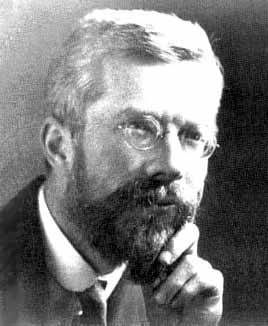
\includegraphics[width=\linewidth]{Fischer.jpg}
    \end{wrapfigure}
     %https://upload.wikimedia.org/wikipedia/commons/4/46/R._A._Fischer.jpg
    Рональд Фишер в 1936 году продемонстрировал работу разработанного им метода анализа.\vspace{1cm}\\
    Данные были собраны американским ботаником Эдгаром Андерсоном.
\end{frame}

\begin{frame}
    \frametitle{\insertsection} 
    \framesubtitle{\insertsubsection}
    Признаки:
    \begin{itemize}
        \item Длина наружной доли околоцветника (англ. sepal length);
        \item Ширина наружной доли околоцветника (англ. sepal width);
        \item Длина внутренней доли околоцветника (англ. petal length);
        \item Ширина внутренней доли околоцветника (англ. petal width).
    \end{itemize}
\end{frame}

\begin{frame}[plain,c]
    \frametitle{\insertsection} 
    \framesubtitle{\insertsubsection}
    \begin{center}
        \huge Примеры кода
    \end{center}
\end{frame}

\section{Кластеризация}
\subsection{Определение}

\begin{frame}
    \frametitle{\insertsection} 
    \framesubtitle{\insertsubsection}    
    \begin{wrapfigure}{l}{0.33\textwidth}
        \vspace{-0.5cm}
        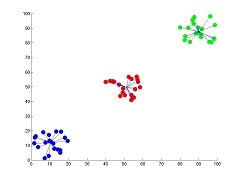
\includegraphics[width=\linewidth]{k-means.jpg}
    \end{wrapfigure}
    % https://sites.google.com/site/dataclusteringalgorithms/k-means-clustering-algorithm
    Кластерный анализ (англ. cluster analysis) — многомерная статистическая процедура, выполняющая сбор данных, содержащих информацию о выборке объектов, и затем упорядочивающая объекты в сравнительно однородные группы.\cite{wiki:clustering_def}
\end{frame}

\section{Визуализация}
\subsection{Набор ирисов Фишера}

\begin{frame}
	\frametitle{\insertsection} 
	\framesubtitle{\insertsubsection}
	\begin{columns}
		\begin{column}[t]{0.3\linewidth}
			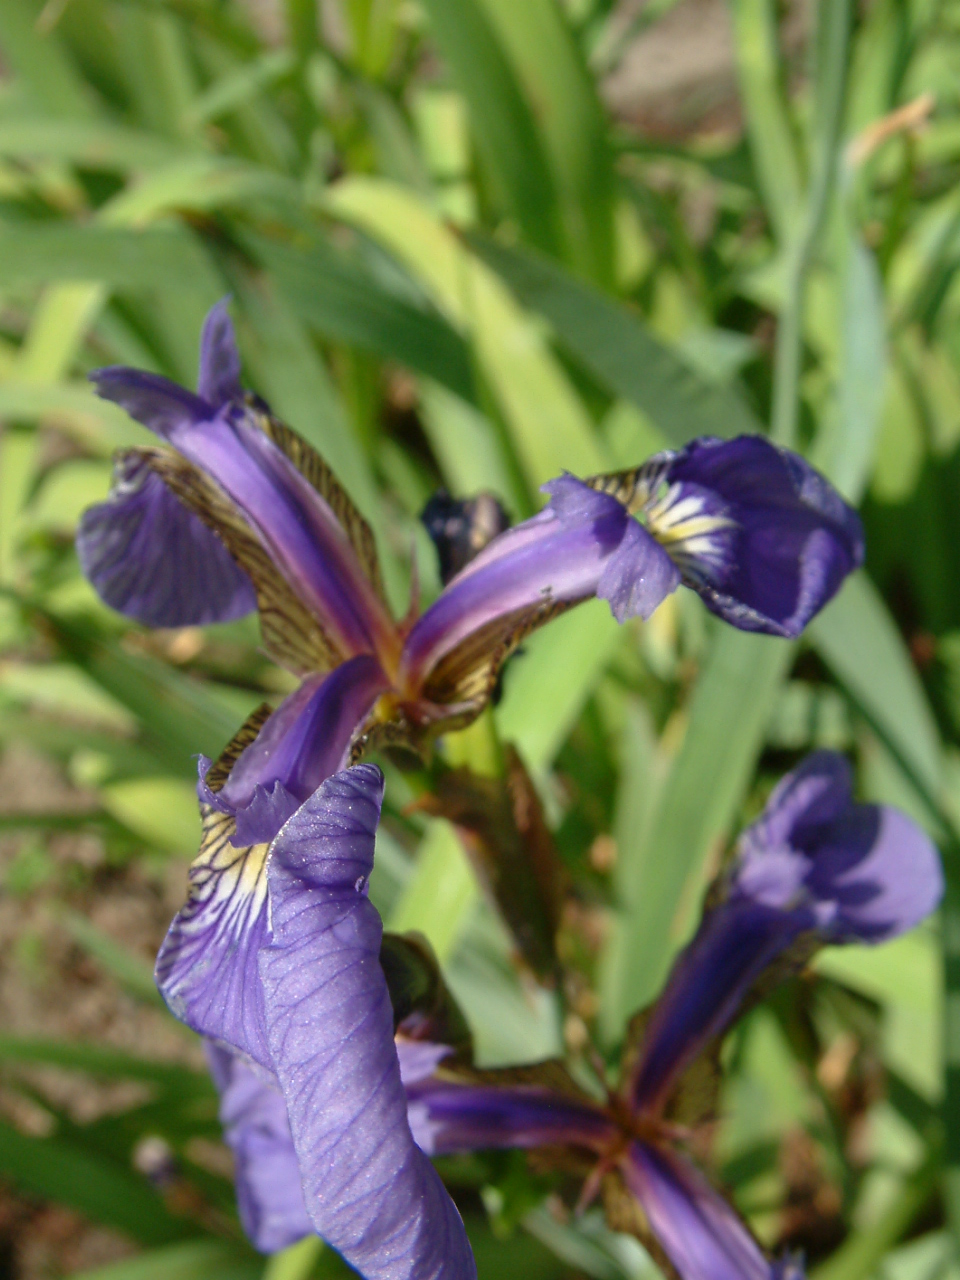
\includegraphics[height=5cm, width=4.5cm]{Iris_setosa.jpg}
			\begin{itemize}
				\item 	Ирис щетинистый (лат. Iris setosa)
			\end{itemize}
		\end{column}	
		\begin{column}[t]{0.3\linewidth}
			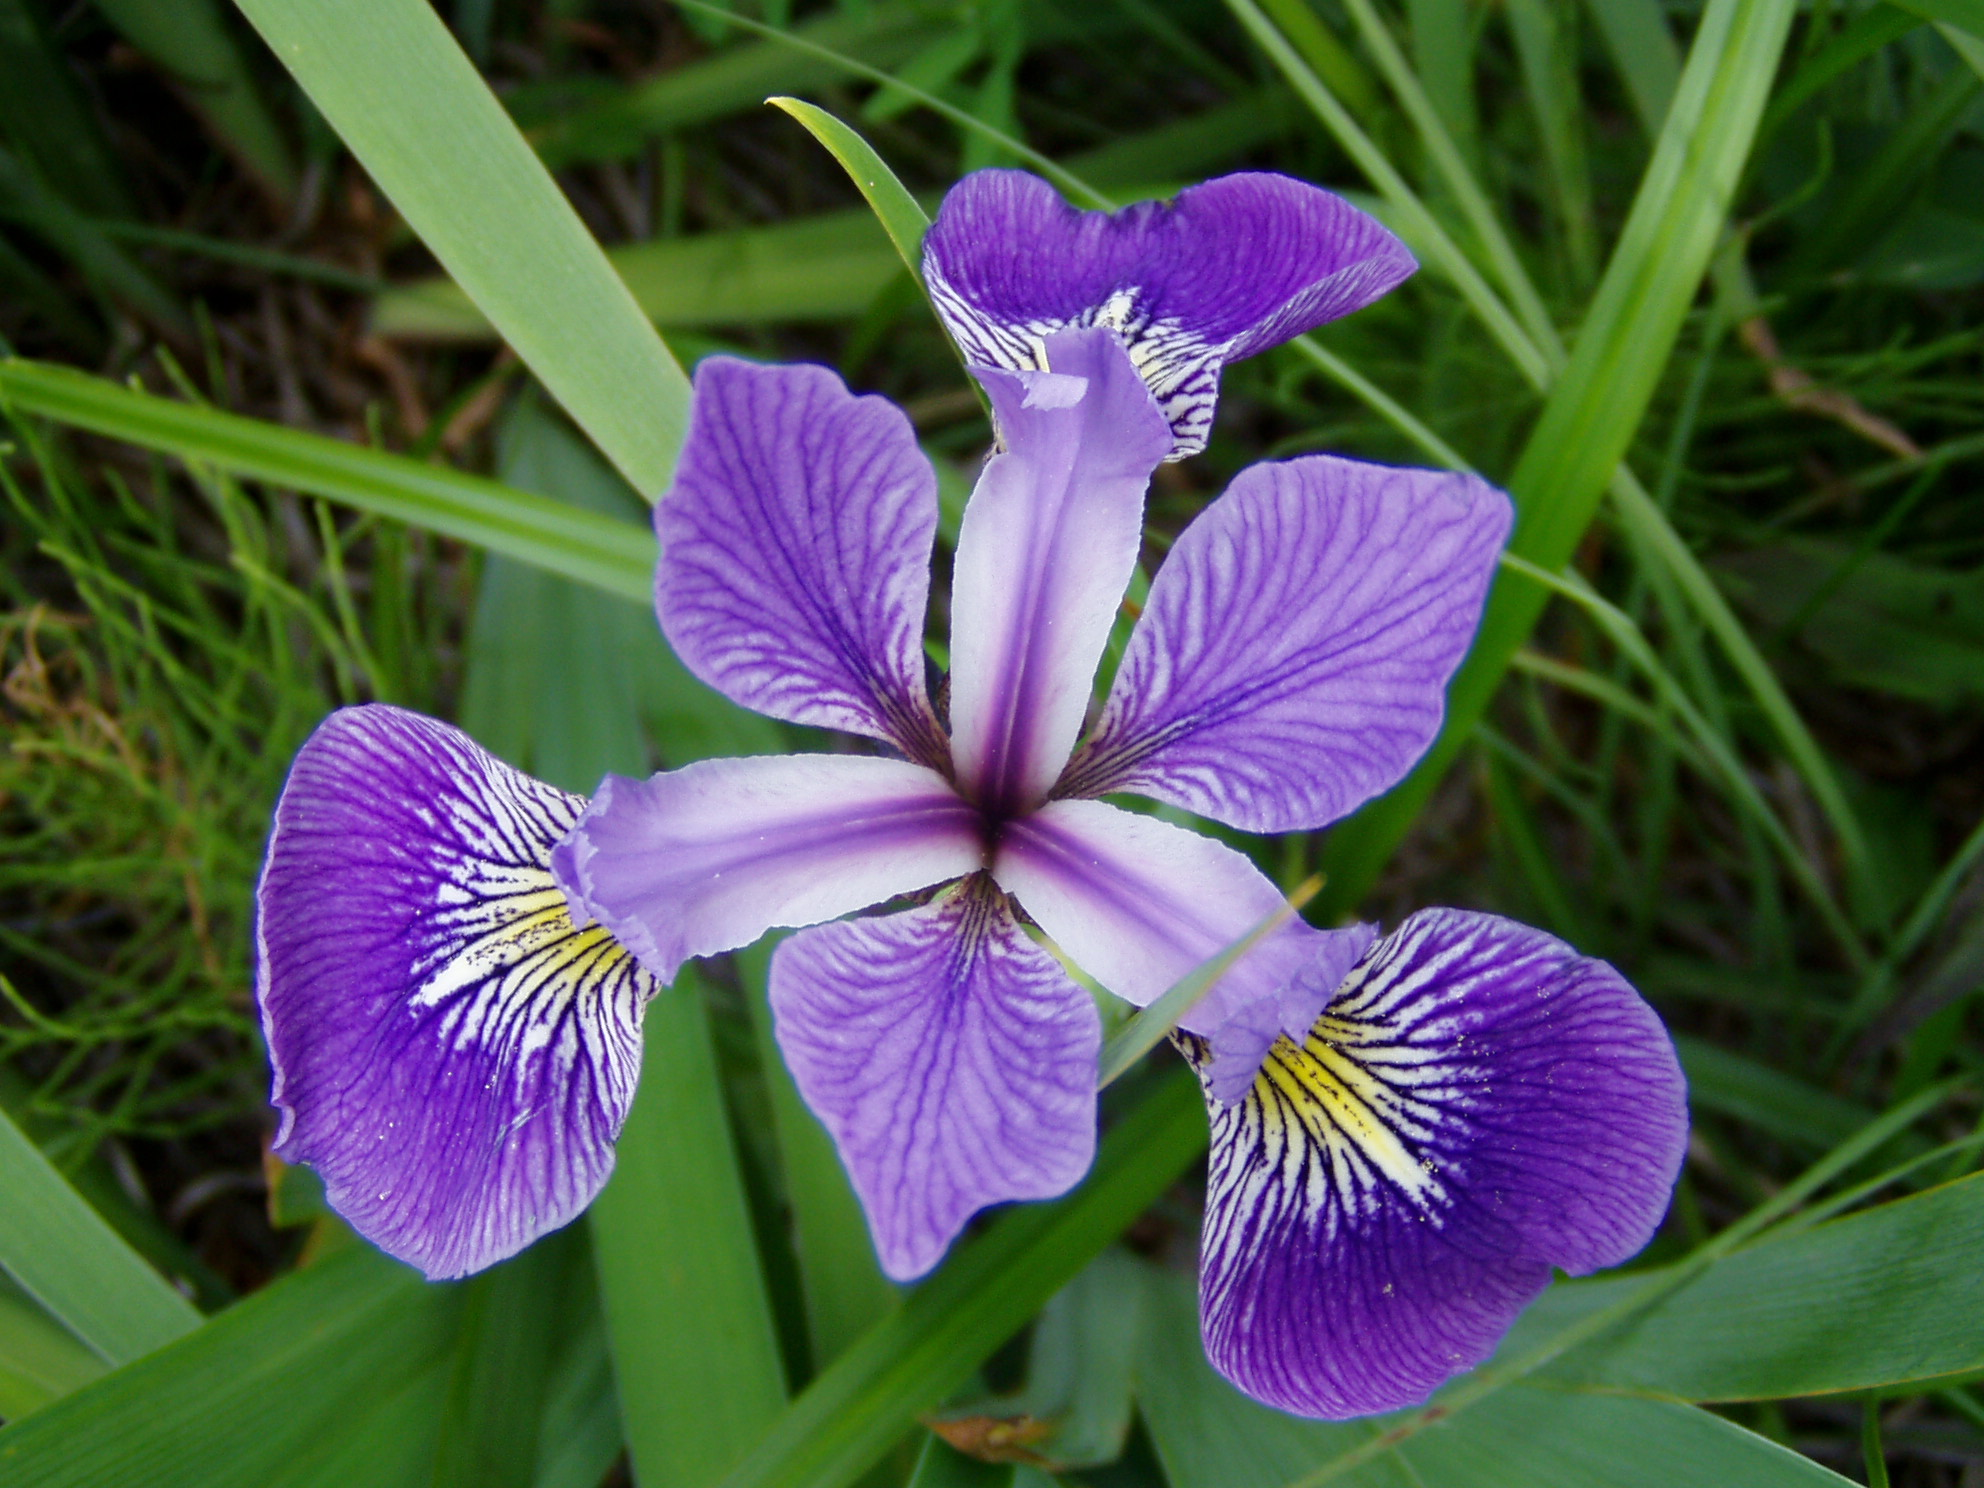
\includegraphics[height=5cm, width=4.5cm]{Iris_versicolor.jpg}
			\begin{itemize}
				\item Iris versicolor
			\end{itemize}
		\end{column}
   		\begin{column}[t]{0.3\linewidth}
   			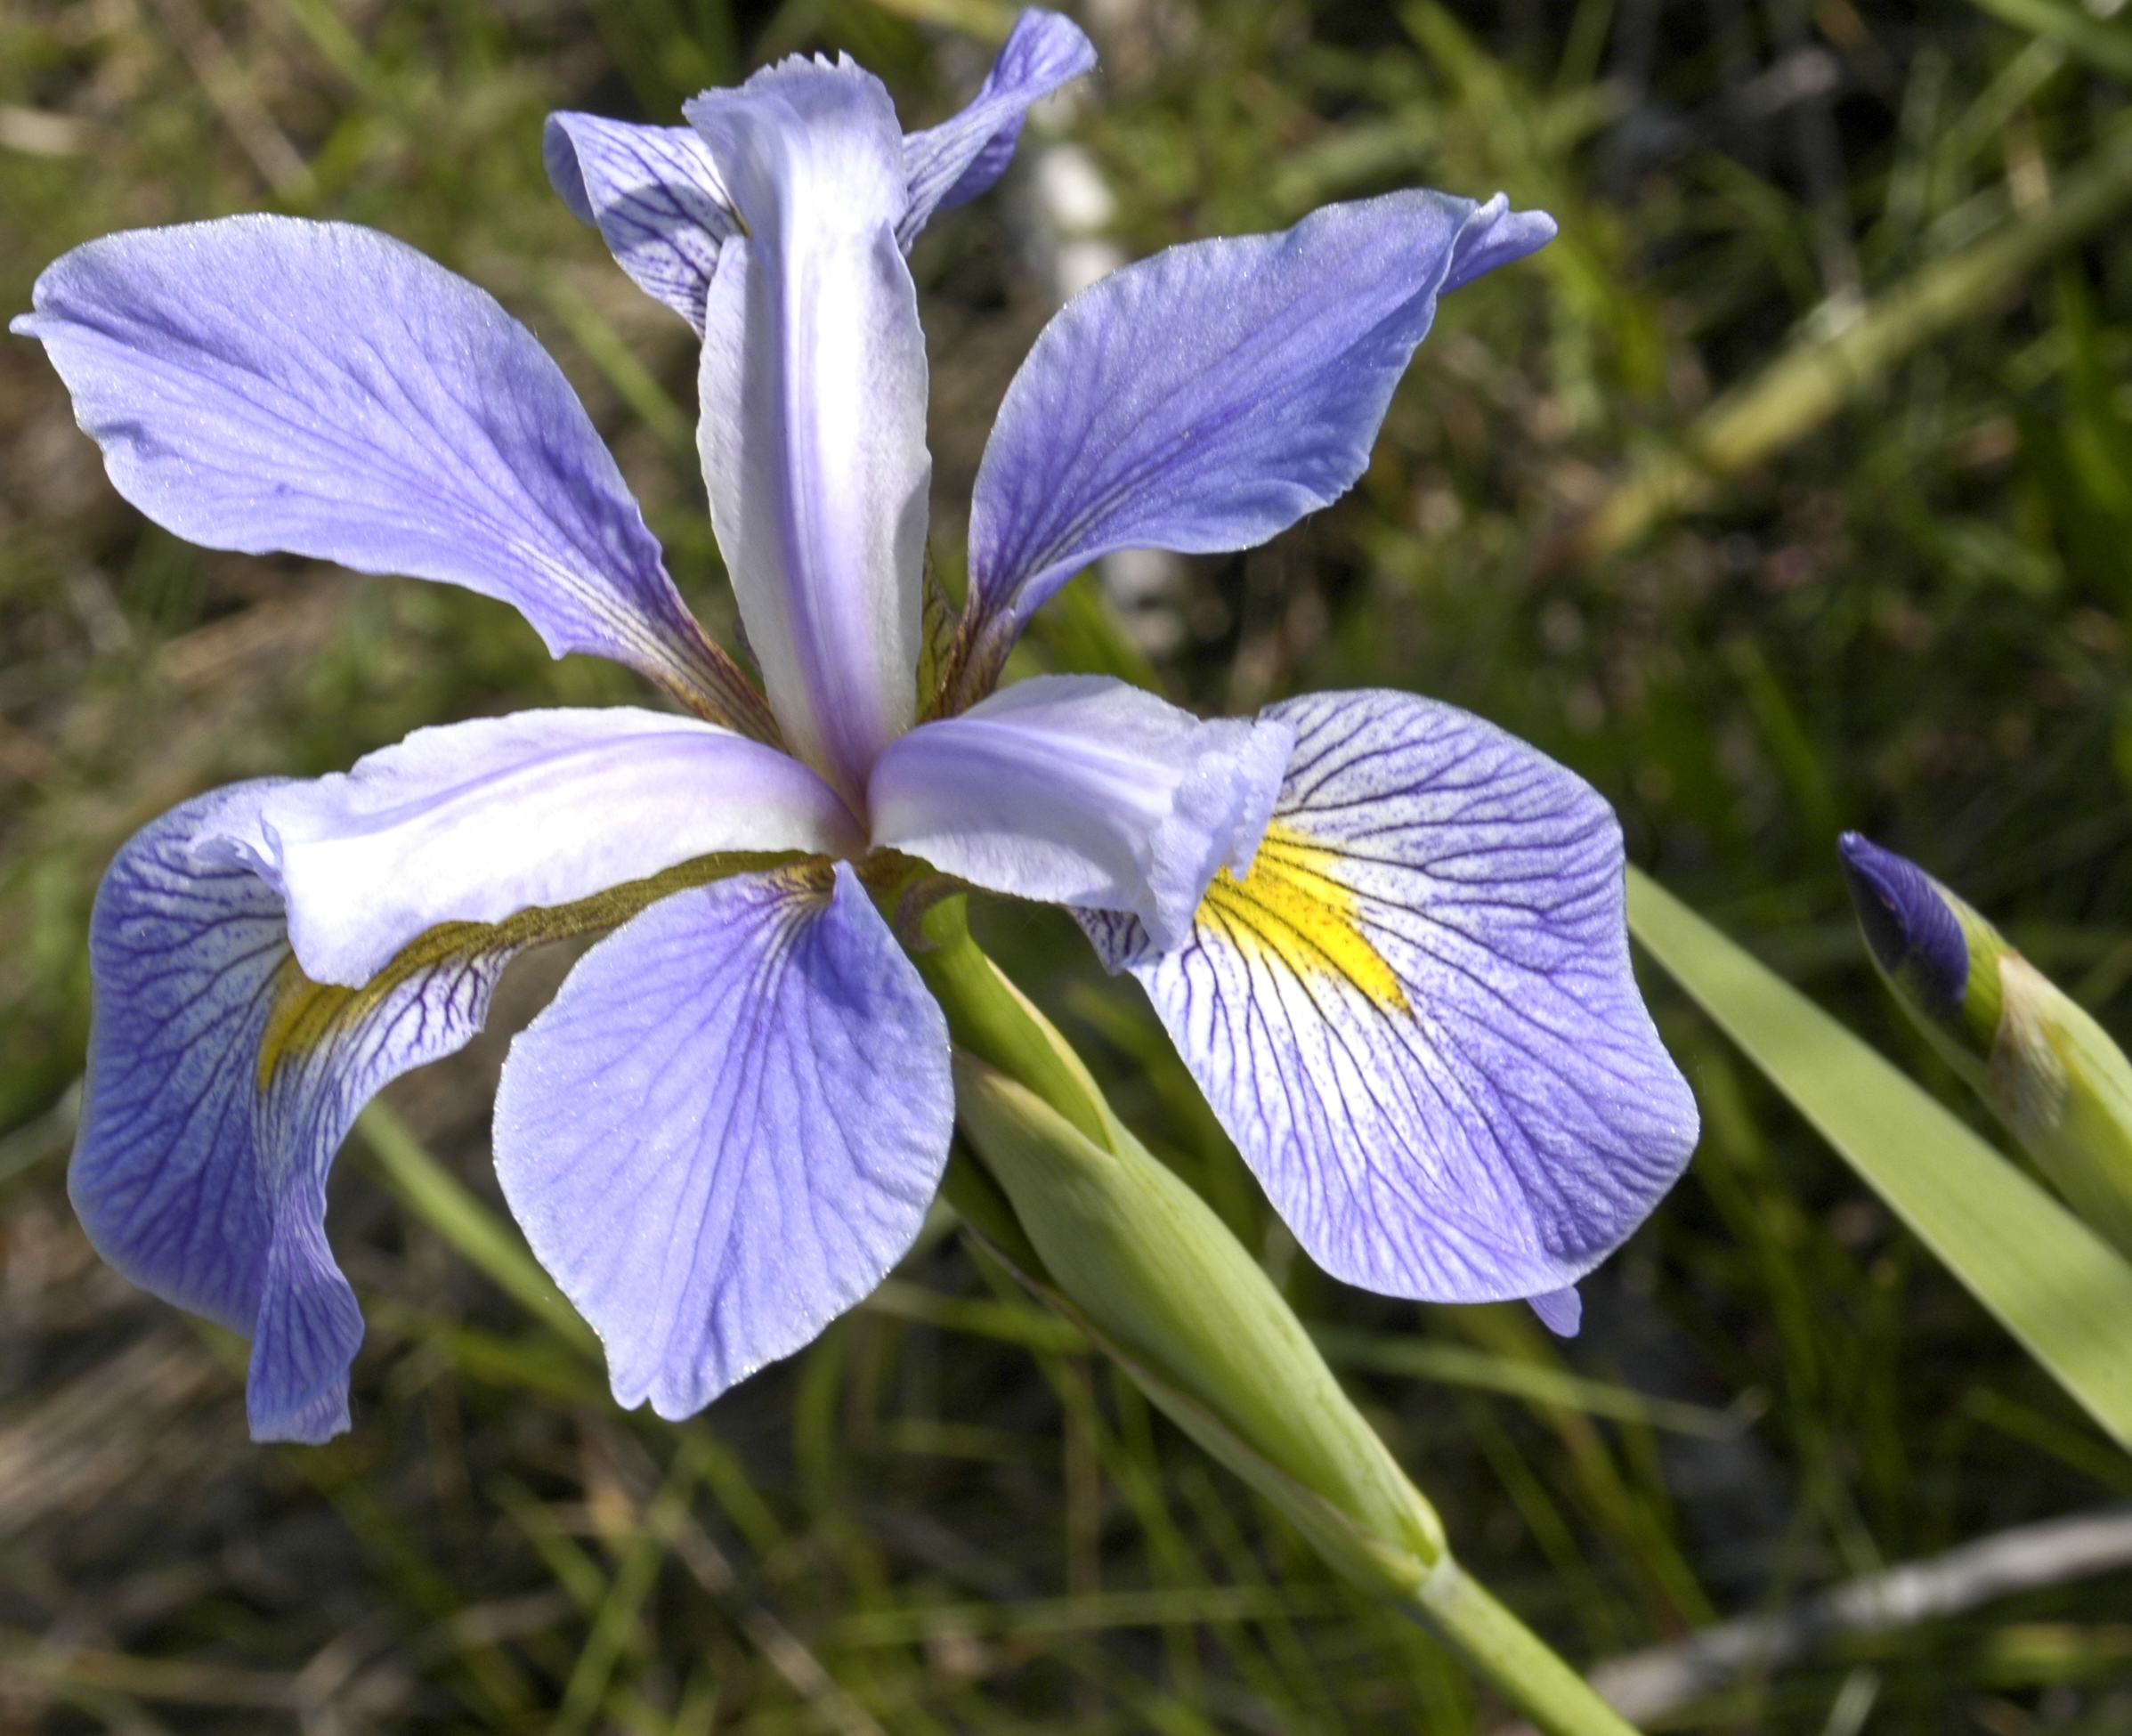
\includegraphics[height=5cm, width=4.5cm]{Iris_virginica.jpg}
   			\begin{itemize}
   				\item Iris virginica
   			\end{itemize}
   		\end{column}
	\end{columns}
\end{frame}

\begin{frame}[plain,c]
    \frametitle{\insertsection} 
    \framesubtitle{\insertsubsection}
    \begin{center}
        \huge Примеры кода
    \end{center}
\end{frame}

\begin{frame}
    \frametitle{\insertsection} 
    \framesubtitle{\insertsubsection}
    Задание:
    \begin{itemize}
        \item Выбрать любые две пары признаков
        \item Отобразить на одном рисунке две зависимости
        \item Подписать график и оси
        \item Добавить легенду.
    \end{itemize}
\end{frame}

\section{Кластеризация}
\subsection{Методы}

\begin{frame}
    \frametitle{\insertsection} 
    \framesubtitle{\insertsubsection}
    \fullframeimage{cluster_comparison.png} % http://scikit-learn.org/stable/modules/clustering.html
\end{frame}

\begin{frame}
    \frametitle{\insertsection} 
    \framesubtitle{\insertsubsection}
    \begin{itemize}
        \item Иерархический (Hierarchical)
        \item K-средних (K-means)
    \end{itemize}
\end{frame}

\subsection{Иерархическая кластеризация}

\begin{frame}
    \frametitle{\insertsection} 
    \framesubtitle{\insertsubsection}
    \begin{wrapfigure}{l}{0.33\textwidth}
        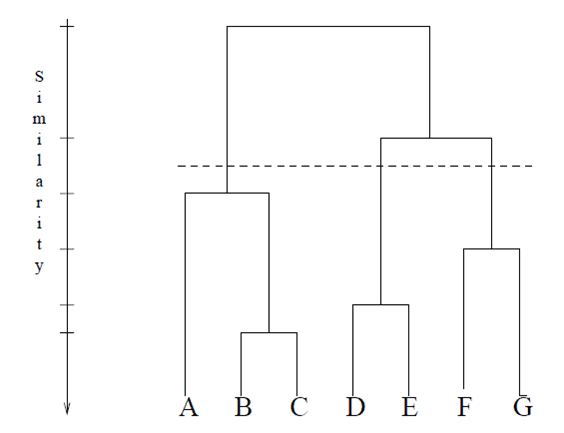
\includegraphics[width=\linewidth]{Agglomerative_clustering_dendogram.png} % https://commons.wikimedia.org/wiki/File:Agglomerative_clustering_dendogram.png
    \end{wrapfigure}
    Определение на пальцах:\\
    Совокупность множеств, одно множество могут полностью лежать в другом множестве, множества не пересекаются.
\end{frame}

\begin{frame}
    \frametitle{\insertsection} 
    \framesubtitle{\insertsubsection}
    \begin{itemize}
        \item Агломеративные методы (основаны на слиянии кластеров)
        \item Дивизимные методы  (основаны на разделении кластеров)
    \end{itemize}
\end{frame}

\subsection{Алгоритм Ланса-Уильямса}

\begin{frame}
    \frametitle{\insertsection} 
    \framesubtitle{\insertsubsection}
    \begin{enumerate}
        \item Создать для каждого объекта свой уютный кластер.
        \item Слить два самых близких кластера в один.
        \item Повторять пред. шаг пока не останется только один кластер.
    \end{enumerate}   
    В результате получаем дендрограмму, определить оптимальное число кластеров можно по ней, взяв то число кластеров, при котором расстояние между ними максимально (обозначается высотой линии на дендрограмме).
\end{frame}

\begin{frame}
    \frametitle{\insertsection} 
    \framesubtitle{\insertsubsection}
    \fullframeimage{Iris_dendrogram.png} % https://commons.wikimedia.org/wiki/File:Iris_dendrogram.png
\end{frame}

\subsection{Достоинства и недостатки}

\begin{frame}
    \frametitle{\insertsection} 
    \framesubtitle{\insertsubsection}
    \begin{itemize}
        \item[+] Строит детальную кластерную структуру (дендрограмму).
        \item[+] Гибкость и удобство настройки.
        \item[--] Квадратичная сложность.
    \end{itemize}
\end{frame}

\subsection{К-средних}

\begin{frame}
    \frametitle{\insertsection} 
    \framesubtitle{\insertsubsection}    
    \begin{enumerate}
        \item Случайно задать центры кластеров.
        \item Найти для каждого объекта свой кластер.
        \begin{enumerate}
            \item Для каждого объекта вычисляем расстояние до каждого из центров кластеров.
            \item Относим объект к тому кластеру, у которого это расстояние минимально.
        \end{enumerate} 
        \item Пересчитать центры кластеров.
        \begin{enumerate}
            \item Для каждого объекта посчитать расстояние до всех остальных объектов в этом кластере.
            \item Назначить центром тот объект у которого максимальное расстояние до объекта того же кластера минимально.
        \end{enumerate} 
        \item Повторять шаги 2-4 до тех пор, пока центры кластеров не перестанут смещаться.
    \end{enumerate}   
\end{frame}

\subsection{Достоинства и недостатки}

\begin{frame}
    \frametitle{\insertsection} 
    \framesubtitle{\insertsubsection}
    \begin{itemize}
        \item[--] Чувствителен к выбору начального приближения.
        \item[--] Необходимо указывать число кластеров как параметр.
        \item[+] Быстро сходится (находит решение).
        \item[+] Прост и нагляден.
        \item[+] Популярен (встроен во многие библиотеке, просто найти информацию, существует множество модификаций).
    \end{itemize}
\end{frame}

\subsection{Оценки сложности}

\begin{frame}
    \frametitle{\insertsection} 
    \framesubtitle{\insertsubsection}
    \begin{center}        
        \begin{tabular}{|c|c|}
            \hline Алгоритм & Вычислительная сложность \\ 
            \hline Иерархический & $O(n^2)$ \\ 
            \hline k-средних & $O(nkl)$, где $k$ – число кластеров, $l$ – число итераций \\ 
            \hline 
        \end{tabular} 
    \end{center}
\end{frame}

\section{Машинное обучение}
\subsection{Определение}

\begin{frame}
    \frametitle{\insertsection} 
    \framesubtitle{\insertsubsection}
    Машинное обучение (англ. machine learning, ML) — класс методов искусственного интеллекта, характерной чертой которых является не прямое решение задачи, а обучение в процессе применения решений множества сходных задач. Для построения таких методов используются средства математической статистики, численных методов, методов оптимизации, теории вероятностей, теории графов, различные техники работы с данными в цифровой форме\cite{wiki:ml_def}.
    
    \vspace{1cm}
    Алгоритм $A$ обучается с эффективностью $E$ над данными $D$, если про росте мощности $|D|$, $E$ проявляет тенденцию к увеличению.
\end{frame}


\section{Список литературы}
\begin{frame} 
    \frametitle{\insertsection}  
    \printbibliography
\end{frame}


\end{document}